\chapter{The Algorithm}

\section{Reference transformation}

The first step of the algorithm lies in transforming a reference sequence covering the selected active region into a De Bruin-like graph. The idea behind this step is very similar to other assembly algorithms based on De Bruin graphs. 

The reference is divided into k-mers, each overlaps with the adjacent ones by k-1 bases. K-mers representing the same sequence are differentiated by their context number, so each k-mer derived from the reference is unique. Two extra k-mers, denoting the beginning and te end of the active region are added to the set. Then, each k-mer is represented by a single vertex in the graph, and edges are defined by the order of the k-mers within the active region.

Formaly speaking, with the active region of length $l$ as represented as a sequence of bases $(b_0, ..., b_{l-1})$, k-mers $K_0, ..., K_{l-k+2}$ are derived from the region as follows:
\begin{itemize}
\item $K_0 = ((B, b_0, ..., b_{k-2}), 0)$
\item $K_1 = ((b_0, ..., b_{k-1}), 0)$
\item . . .
\item $K_i = ((b_i, ..., b_{i+k-1}), c_i), 2 <= i <=  l-k+1$
\item . . .
\item $K_{l-k+2} = ((b_{l-2k+3}, ..., b_{l-k+1}, E), 0)$
\end{itemize}
$c_i$ represents the context number of the k-mer $K_i$. The number is set to zero for k-mers the sequence of which do not repeat within the active region. On the other hand, let's assume that k-mers $K_{i_0}, ..., K_{i_{n-1}}, i_0 < ... < i_{n-1}$ represent the same sequence. Their context number is defined as
$$
c_{i_j} = j, 
$$

$K_0$ and $K_{l-k+2}$ are special k-mers added to the set in order to show the start and end of the active region within the graph. $B$ and $E$ are virtual bases that ensures these k-mers represent unique sekquences. The bases must not appear in the active region.

After their derivation, each k-mer $K_i$ is transformed into a single vertex $v_i$. Edges follow the order the k-mers occurrs within the active region. In other words, the edge set of the graph is
$$
E = {(v_i, v_{i+1})}, 0 <= i <= l-k+1
$$

Figure \ref{fig:ref-my} displays a graph created by transformation of an active region \texttt{ATCTGTATATATG} with k-mer size of 5. The algorithm derives the following k-mers:
$$
K_0 = ((B, A, T, C, T), 0)
K_1 = ((A, T, C, T, G), 0)
K_2 = ((T, C, T, G, T), 0)
K_3 = ((C, T, G, T, A), 0)
K_4 = ((T, G, T, A, T), 0)
K_5 = ((G, T, A, T, A), 0)
K_6 = ((T, A, T, A, T), 0)
K_7 = ((A, T, A, T, A), 0)
K_8 = ((T, A, T, A, T), 1)
K_9 = ((A, T, A, T, G), 0)
K_{10} = ((T, A, T, G, E), 0)
$$

As can bee seen, there are two k-mers representing sequence \texttt{TATAT}, namely $K_6$ and $K_8$. Because of their distinct context number, their are represented by separate vertices. Introduction of the numbers removed a loop from the graph. The loop can be observed on Figure \ref{fig:ref-db} that shows a classical De Bruin graph constructed from the same active region. K-mers $K_6$ and $K_8$ are represented by the same vertex. In order to recover the sequence, it is required to know how many times the loop was actually used during the transformation step.

\begin{figure}
	\centering
	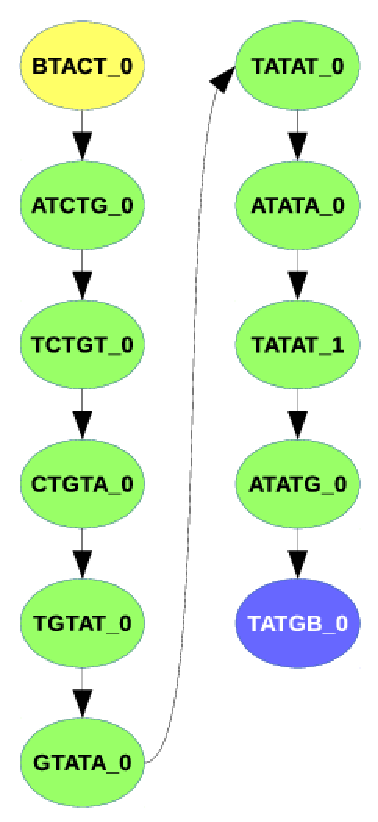
\includegraphics{img/ref-my.pdf}
	\caption{Graph resulting from the transformation of \texttt{ATCTGTATATATG} sequence}
	\label{fig:ref-my}
\end{figure}

\begin{figure}
	\centering
	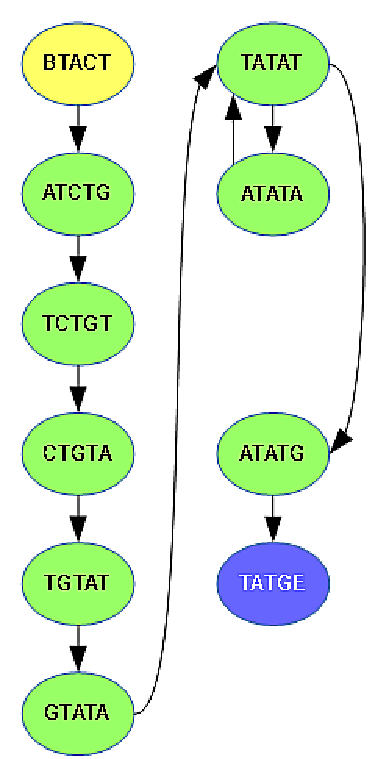
\includegraphics{img/ref-db.pdf}
	\caption{Transformation of the ATCTGTATATATG squence to a standard De Bruin graph (with no k-mer context numbers)}
	\label{fig:ref-db}
\end{figure}

Although we solved the loop problem, for now, by not allowing them to appear, and thus making the graph, at this stage, linear, things get more complicated in the next step that covers introducing individual reads into the graph.

\section{Adding Reads}

